% Created 2021-09-09 Thu 15:43
% Intended LaTeX compiler: pdflatex
\documentclass[11pt]{article}
\usepackage[utf8]{inputenc}
\usepackage{afterpage}
\usepackage[left=1.5in,right=1in]{geometry}
\usepackage{subcaption}
\usepackage[T1]{fontenc}
\usepackage{graphicx}
\usepackage{grffile}
\usepackage{longtable}
\usepackage{wrapfig}
\usepackage{rotating}
\usepackage[normalem]{ulem}
\usepackage{amsmath}
\usepackage{textcomp}
\usepackage{amssymb}
\usepackage{capt-of}
\usepackage{hyperref}
\usepackage{tcolorbox}
\newtcolorbox{codebox}{colback=green!5!white,colframe=green!75!black}
\author{Mridul Gupta (AIZ218322)}
\date{Friday 10 September 2021}
\title{COL774 Assignment 1}
\hypersetup{
 pdfauthor={Mridul Gupta (AIZ218322)},
 pdftitle={COL774 Assignment 1},
 pdfkeywords={},
 pdfsubject={},
 pdfcreator={Emacs 27.1 (Org mode 9.3)}, 
 pdflang={English}}
\begin{document}

\maketitle
\section{Q1}
\label{sec:orge4c8fb7}
\subsection{Q1(a)}
\label{sec:org99d1faf}
\begin{codebox}
Run as
\begin{verbatim}
$ python one_a.py --data-x path/to/linearX.csv
--data-y path/to/linearY.csv
\end{verbatim}
\end{codebox}
\begin{enumerate}
\item The first thing I did was look at the data and note how many
lines it was. The input data was 1D and had 100 samples.
\item I wrote a simple code to load the data and plot. And scaled
the data to zero centered and unit variance.
\item I wrote the piece of code to calculate the cost function
and plotted the cost function, keeping one of the \(\theta_i\)
constant at 0 while varying the other. In this way I was able to
find that the optimum parameter was \(\hat{\theta}=[0,1]\).
\item Then, I wrote the gradient calculation step of
gradient descent and combined it with the data loading step.
\item After all the debugging was done, I rewrote the code using
\texttt{dataloader} style syntax to make working easier. The
inspiration was pytorch code I worked on before.
\item I initialized the parameters to \([0,0]\), but the graphs showed
little movement of parameters on the space, to get a dramatic
graph, I made the initialization point far from the actual
values of \([0,1]\).
\item I also experimented with different number of epochs, learning
rates and convergence criteria. Early on, I was using the
convergence of \(\theta^t\) to an epsilon-ball \(\mathbb{B}_{\epsilon}\)
to determine convergence. But later, I settled to using the
convergence of the cost function values over time as convergence criterion.
\end{enumerate}
Learning Rate: 0.001\\
Stopping criteria: \(\lVert J^{t}-J^{t-1}\rVert_2 < 10^{-6}\)\\
Final parameter values: \(\theta_0=0.96503917\) and \(\theta_1=0.0226594\)
\subsection{Q1(b)}
\label{sec:org2e4e985}
\begin{codebox}
Run as
\begin{verbatim}
$ python one_b.py --data-x path/to/linearX.csv
--data-y path/to/linearY.csv
\end{verbatim}
\end{codebox}
\begin{figure}[!ht]
\centering
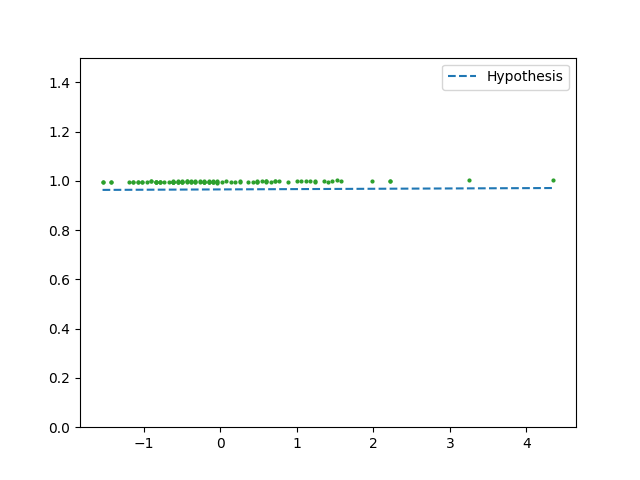
\includegraphics[width=.7\linewidth]{/home/mridul/scai/ml/hw1/src/q1/one_b.png}
\caption{\label{fig:org2bc820c}Data}
\end{figure}
\subsection{Q1(c)}
\label{sec:org2afdae8}
\begin{codebox}
Run as
\begin{verbatim}
$ python one_c.py --data-x path/to/linearX.csv --data-y
path/to/linearY.csv [--no-rotate]
\end{verbatim}
Note that the default animation rotates, this was done to
save frames in a way that the three dimensionality is
visible. This can be disabled using \verb|--no-rotate|
option.\par
\end{codebox}
\noindent The animation cannot be attached here, instead I'm attaching the first
and the final epoch snapshots. See figure \ref{fig:org1c0d57c}-\ref{fig:orgc4a9d5e}.
\begin{figure}[!ht]
\centering
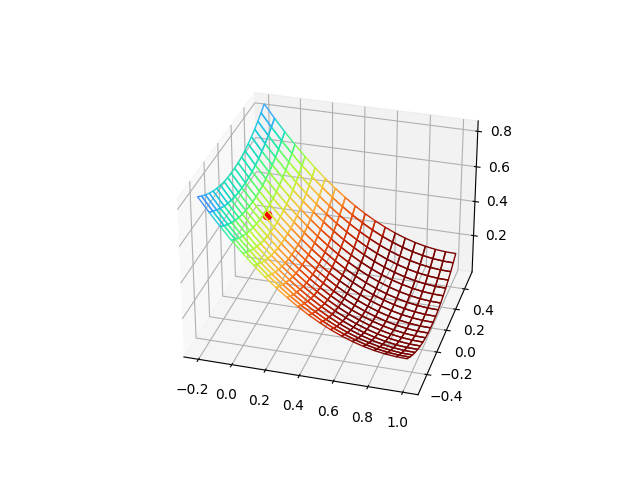
\includegraphics[width=.8\linewidth]{/home/mridul/scai/ml/hw1/src/q1/framessurf/00001.png}
\caption{\label{fig:org1c0d57c}First epoch}
\end{figure}
\begin{figure}[!ht]
\centering
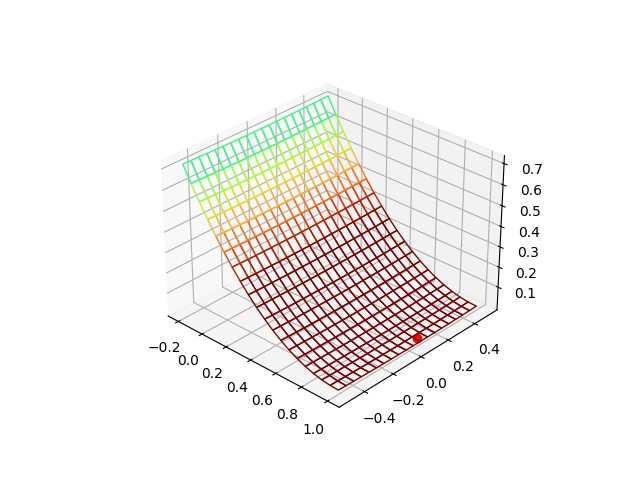
\includegraphics[width=.8\linewidth]{/home/mridul/scai/ml/hw1/src/q1/framessurf/03453.png}
\caption{\label{fig:orgc4a9d5e}Last epoch}
\end{figure}
\afterpage{\clearpage}
\subsection{Q1(d)}
\label{sec:org9368090}
\begin{codebox}
Run as
\begin{verbatim}
$ python one_d.py --data-x path/to/linearX.csv
--data-y path/to/linearY.csv
\end{verbatim}
\end{codebox}
\noindent Again, cannot attach animation here, but attaching animation in the
zip file. See figure \ref{fig:contours}.
\begin{figure}[!ht]
\centering
	\subfloat[First epoch]{%
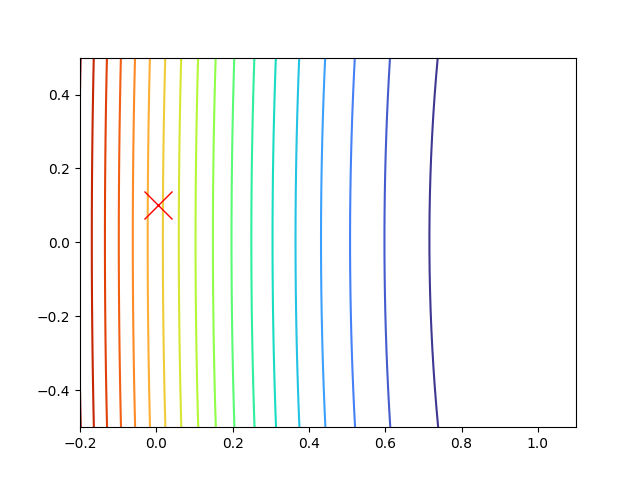
\includegraphics[width=.5\linewidth]{/home/mridul/scai/ml/hw1/src/q1/framescontour/tokeep/0.001_first.png}
	}
	\subfloat[Last epoch]{%
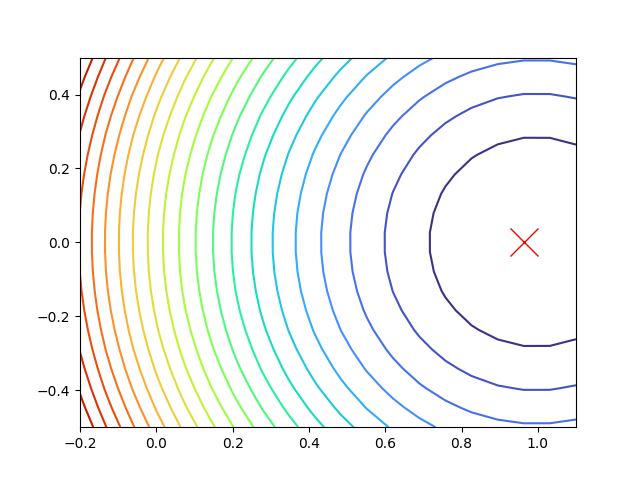
\includegraphics[width=.5\linewidth]{/home/mridul/scai/ml/hw1/src/q1/framescontour/tokeep/0.001_last.png}
	}
	\caption{\label{fig:contours}Contour plot snapshots}
\end{figure}
\subsection{Q1(e)}
\label{sec:org1f48017}
I observe exactly what I'd hope to, the parameters move towards the
optimum faster as the step size grows. See table. The direction of movement is
almost the same, the changes in step size were small so that the
algorithm never diverged.
\begin{center}
\begin{tabular}{rr}
step size & \#epochs before convergence\\
\hline
0.001 & 3454\\
0.025 & 201\\
0.1 & 55\\
\end{tabular}
\end{center}
\begin{figure}[!ht]
\centering
	\subfloat[First epoch 0.001]{%
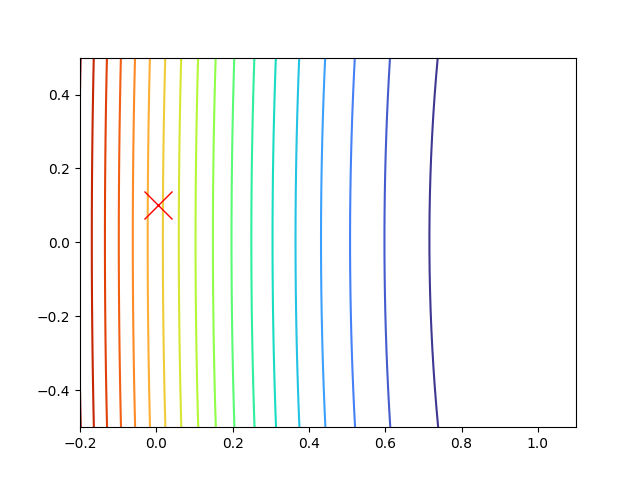
\includegraphics[width=.5\linewidth]{/home/mridul/scai/ml/hw1/src/q1/framescontour/tokeep/0.001_first.png}
	}
	\subfloat[Last epoch 0.001]{%
		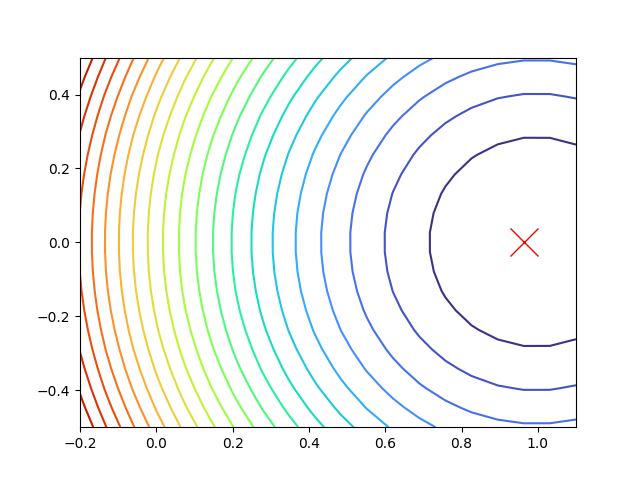
\includegraphics[width=.5\linewidth]{/home/mridul/scai/ml/hw1/src/q1/framescontour/tokeep/0.001_last.png}
	}
	\caption{Contour plot}
\end{figure}
\begin{figure}[!ht]
\centering
	\subfloat[First epoch 0.025]{%
		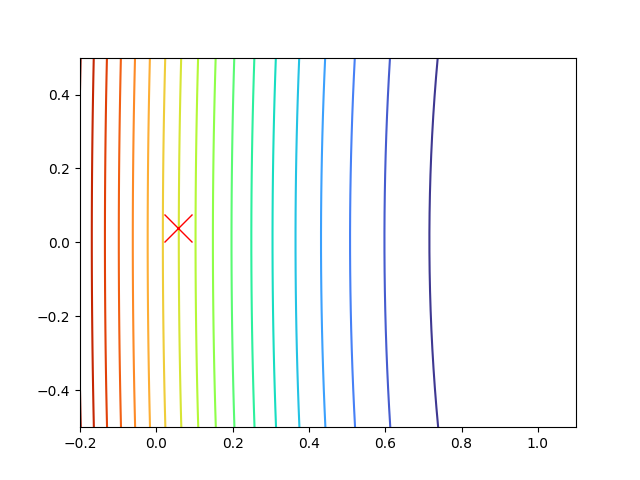
\includegraphics[width=.5\linewidth]{/home/mridul/scai/ml/hw1/src/q1/framescontour/tokeep/0.025_first.png}
	}
	\subfloat[Last epoch 0.025]{%
		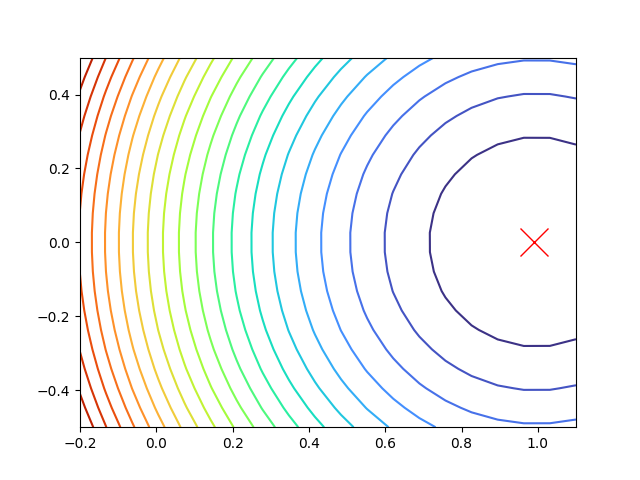
\includegraphics[width=.5\linewidth]{/home/mridul/scai/ml/hw1/src/q1/framescontour/tokeep/0.025_last.png}
	}
	\caption{Contour plot}
\end{figure}
\begin{figure}[!ht]
\centering
	\subfloat[First epoch 0.1]{%
		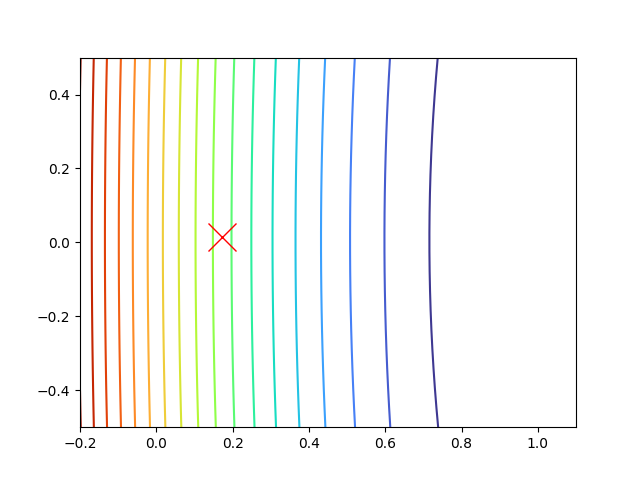
\includegraphics[width=.5\linewidth]{/home/mridul/scai/ml/hw1/src/q1/framescontour/tokeep/0.1_first.png}
	}
	\subfloat[Last epoch 0.1]{%
		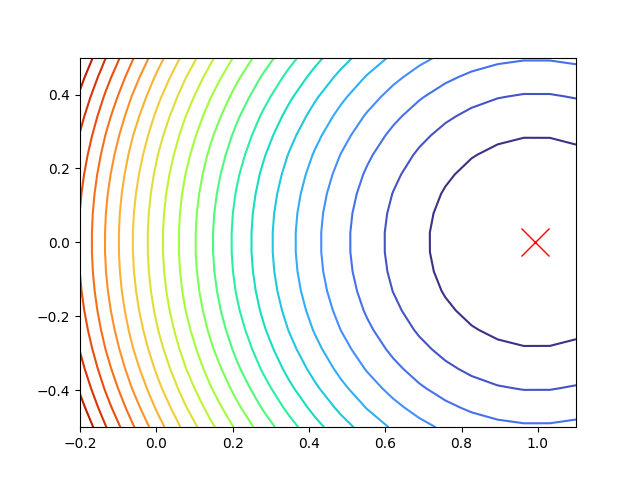
\includegraphics[width=.5\linewidth]{/home/mridul/scai/ml/hw1/src/q1/framescontour/tokeep/0.1_last.png}
	}
	\caption{Contour plot}
\end{figure}
\clearpage
\section{Q2}
\label{sec:orged46b7f}
\subsection{Q2(a)}
\label{sec:orge29d38b}
\begin{codebox}
Run as
\begin{verbatim}
$ python two_a.py
\end{verbatim}
\end{codebox}
\begin{enumerate}
\item I wrote a snippet that takes the theta parameters, the size of
the dataset to generate, the \(\mu_1\), \(\sigma^2_1\), \(\mu_2\),
\(\sigma^2_2\) corresponding to the features \(x_1\) and \(x_2\) and
also the variance of the noise \(\sigma^2_{noise}\). And generates
the dataset \(\{x^{(i)},y^{(i)}\}\) and returns it.
\item A little note, to vectorize the noise adding, the
\(\theta\) is appended with a \(1\) just as \(1\) is added to
the \(x\) data to incorporate the intercept term in it.
\end{enumerate}
\subsection{Q2(b)}
\label{sec:org8ea60f9}
\begin{codebox}
Run as
\begin{verbatim}
$ python two_b.py [--epochs [number-of-epochs]] [--batch-size
[batch-size]] [--eps [epsilon-used-in-convergence]]
\end{verbatim}
Note, all the options are non-mandatory.
\end{codebox}
\begin{enumerate}
\item I wrote the \texttt{DataLoader} class, the \texttt{getdata} function, the
\texttt{get\_dataloader} function, the \texttt{dist} function,
the \texttt{J} function as helper functions.
\item The \texttt{DataLoader} class is now augmented to support
shuffling, and return mini-batches of data.
\item The main stochastic gradient code is in function named
\texttt{two\_b}. It's pretty straight forward. It consists of the
initialization, the outer loop for each epoch and the inner loop
to perform gradient descent on the minibatch. The batch size
component is encapsulated in the \texttt{DataLoader}.
\end{enumerate}
\subsection{Q2(c)}
\label{sec:orgb9ee740}
\begin{codebox}
Run as
\begin{verbatim}
$ python two_c.py --batch-size <batch-size> --test-file
path/to/q2test.csv [--no-skip-first]
\end{verbatim}
The \verb|--no-skip-first| argument relates to the csv file,
whether the first row represent header or data.
\end{codebox}
\begin{center}
\begin{tabular}{rrrr}
\hline
Batch size & \(\theta_0\) & \(\theta_1\) & \(\theta_2\)\\
\hline
1000000 & 2.87880453 & 1.0266891 & 1.99118959\\
10000 & 2.99767533 & 1.00118544 & 1.9995014\\
100 & 2.99932185 & 0.99948737 & 2.00046515\\
1 & 3.00208729 & 1.01619096 & 1.97847073\\
\hline
Original & 3 & 1 & 2\\
\hline
\end{tabular}
\end{center}

\begin{center}
\begin{tabular}{rrrr}
\hline
Deltas & \(\theta_0\) & \(\theta_1\) & \(\theta_2\)\\
\hline
1000000 & 0.12119547 & 0.0266891 & 0.00881041\\
10000 & 0.00232467 & 0.00118544 & 0.0004986\\
100 & 0.00067815 & 0.0051263 & 0.00046515\\
1 & 0.00208729 & 0.01619096 & 0.02152927\\
\hline
\end{tabular}
\end{center}

\begin{center}
\begin{tabular}{rrrr}
\hline
Percentage & \(\theta_0\) & \(\theta_1\) & \(\theta_2\)\\
\hline
1000000 & 4.04 & 2.67 & 0.44\\
10000 & 0.08 & 0.11 & 0.02\\
100 & 0.02 & 0.51 & 0.02\\
1 & 0.07 & 1.62 & 1.08\\
\hline
\end{tabular}
\end{center}

\begin{center}
\begin{tabular}{rr}
\hline
Batch size & Euclidean
norm of \%ages\\
	&seen as a vector \\
\hline
1000000 & 4.86\\
10000 & 0.14\\
100 & 0.51\\
1 & 1.95\\
\hline
\end{tabular}
\end{center}

\begin{center}
\begin{tabular}{rr}
Batch Size & MSE on test set\\
\hline
1000000 & 1.0261181852211296\\
10000 & 0.9830393147537965\\
100 & 0.9829447376744409\\
1 & 1.0225014963300452\\
Original \(\theta\) & 0.9829469214999982\\
\end{tabular}
\end{center}

\begin{center}
\begin{tabular}{rrr}
\hline
Batch size & Epochs & Iterations\\
\hline
1000000 & 11500 & 11500\\
\hline
10000 & 240 & 24000\\
\hline
100 & 20 & 200000\\
(did not converge) &  & \\
\hline
1 & <1 & 83000\\
\hline
\end{tabular}
\end{center}

The speed of convergence was ordered like this for batch sizes:
\(10000<1<1000000<100^*\) (convergence was not reached for batch size 100.)
\subsection{Q2(d)}
\begin{codebox}
Run as
\begin{verbatim}
$ python two_d.py --batch-size <batch-size> [--start-skip
[iteration number]] [--skip-frame [number of frames to
skip]] [--sleep [sleep duration]] [-s]
[--stop-at [stop iteration number]]
\end{verbatim}
\begin{description}
	\item[--start-skip] Since the parameter
		movement starts slowing, skipping some
		frames makes the movement visible to eye,
		this argument tells which iteration to start
		skipping from
	\item[--skip-frame] This tells how many
		frames to skip
	\item[--sleep] The sleep duration between
		each frame plot
	\item[-s] Save plots to directory named
		frames in the same folder as the
		code, to create animation with ffmpeg.
	\item[--stop-at] Since the movements towards
		the end get really slow and imperceptible,
		this helps stop the animation early, also
		helpful while saving frames.
\end{description}
\end{codebox}
\label{sec:orgcee7e86}
In the cost, we are basically performing sample mean of the squared
errors. This is the number we want to minimize. And thus the gradient
is also the sample mean of derivatives of squared error (in this case
because the hypothesis does not create complex combinations of
features).\par
The sample mean converges to the population mean as the sample size
goes to \(\infty\) according to weak law of large numbers.\par
\textbf{Weak Law of Large Numbers}:
\(\displaystyle\lim_{n\rightarrow\infty}P(\lvert\bar{x_n}-\mu\rvert>\varepsilon)=0\)
for all \(\varepsilon > 0\).\par
This means that the approximation to the gradient gets smoother as the
batch size increases. Which is visible in the smoothness of the path
the parameters take as batch size increases. But this
better approximation comes at the added cost of calculations. And as
the batch size goes up, the number of updates to \(\theta\) goes down
per epoch, and more epochs are needed. Each epoch operates once on the
whole data, thus the time taken is huge.
\begin{figure}[!ht]
\centering
\subfloat[Batch size = 1]{%
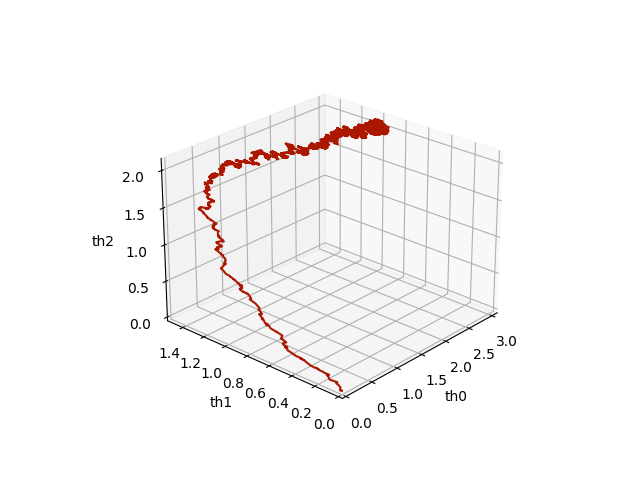
\includegraphics[width=.5\linewidth]{/home/mridul/scai/ml/hw1/src/q2/frames/0000001_000000951.png}
}
\subfloat[Batch size = 100]{%
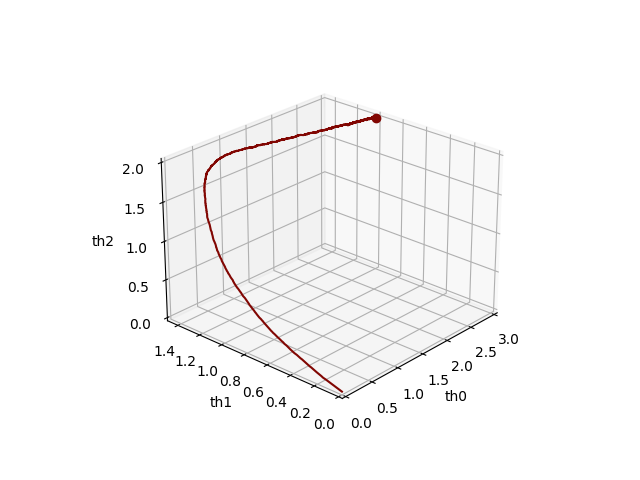
\includegraphics[width=.5\linewidth]{/home/mridul/scai/ml/hw1/src/q2/frames/0000100_000000441.png}
}
\caption{Parameter movement curve}
\end{figure}
\begin{figure}[!ht]
\centering
\subfloat[Batch size = 10000]{%
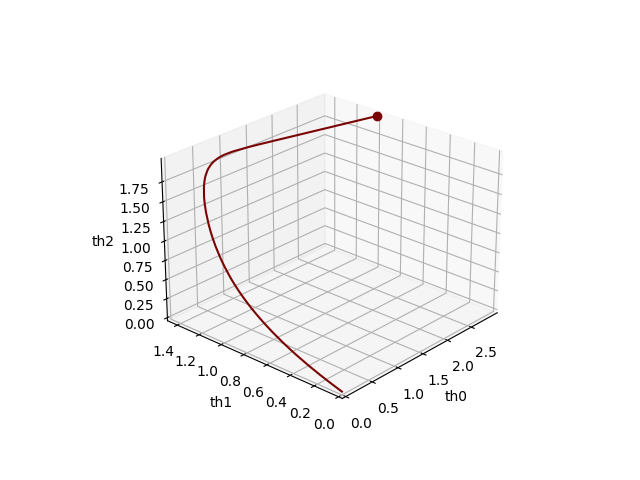
\includegraphics[width=.5\linewidth]{/home/mridul/scai/ml/hw1/src/q2/frames/0010000_000000872.png}
}
\subfloat[Batch size = 1000000]{%
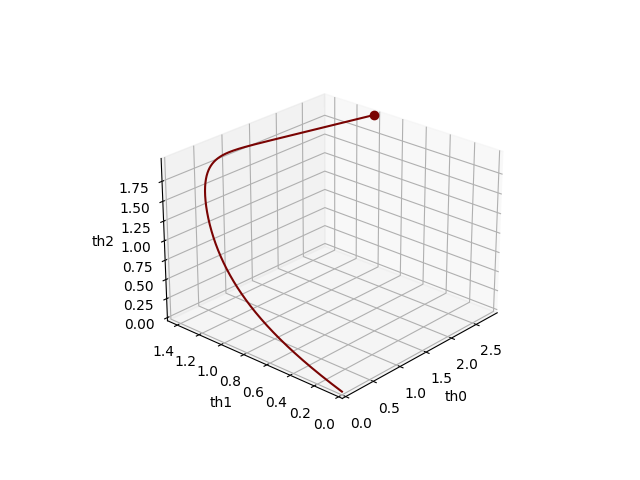
\includegraphics[width=.5\linewidth]{/home/mridul/scai/ml/hw1/src/q2/frames/1000000_000000622.png}
}
\caption{Parameter movement curve}
\end{figure}
	\begin{figure}[!htb]
		\begin{tabular}{cc}
			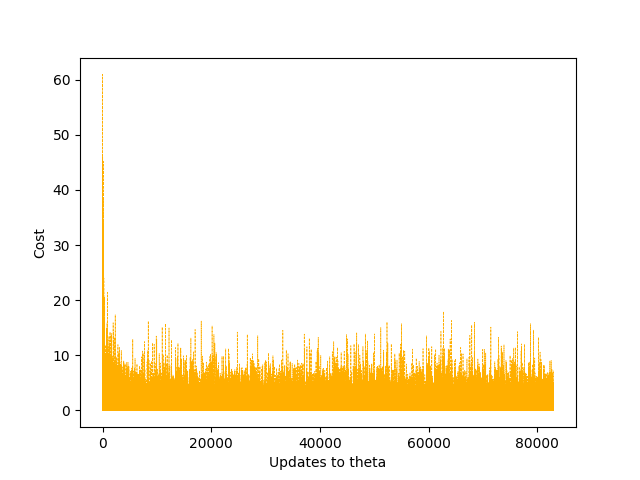
\includegraphics[width=75mm]{/home/mridul/scai/ml/hw1/src/q2/Js1.png} & 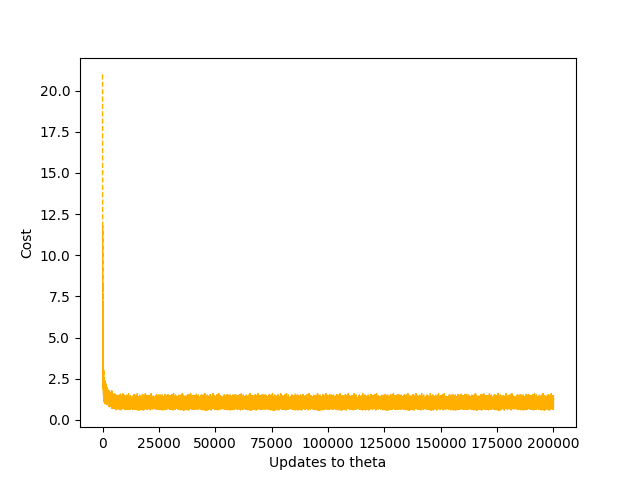
\includegraphics[width=75mm]{/home/mridul/scai/ml/hw1/src/q2/Js2.png}\\
			(a) Batch size: 1 & (b) Batch size 100\\
			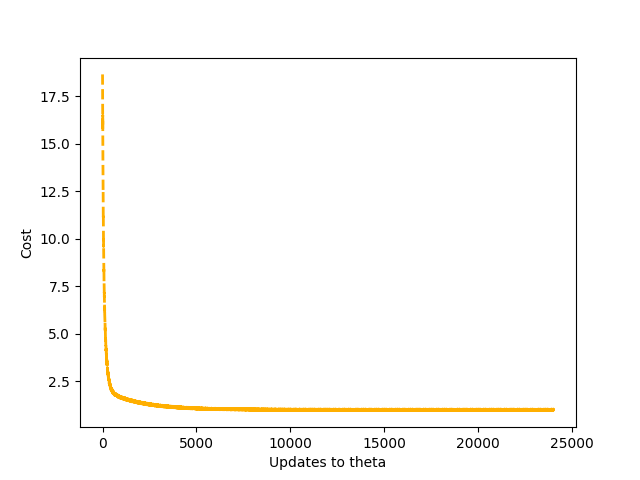
\includegraphics[width=75mm]{/home/mridul/scai/ml/hw1/src/q2/Js3.png} & 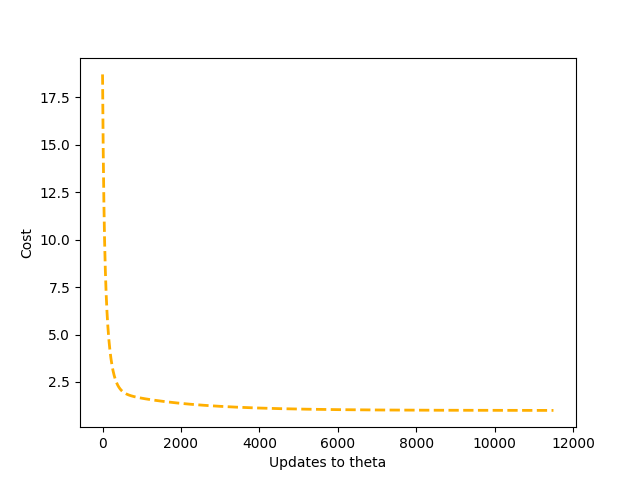
\includegraphics[width=75mm]{/home/mridul/scai/ml/hw1/src/q2/Js4.png}\\
			(c) Batch size: 10000 & (d) Batch size 1000000\\
		\end{tabular}
		\caption{Learning curves}
	\end{figure}
\section{Q3}
\label{sec:org8d5b946}
\subsection{Q3(a)}
\label{sec:orgc5c465e}
\begin{codebox}
Run as
\begin{verbatim}
$ python three_a.py --data-x path/to/logisticX.csv --data-y
path/to/logisticY.csv
\end{verbatim}
\end{codebox}
\begin{equation}
\ell(\theta;x,y)=\sum_{i=1}^m\bigl(y^{(i)}\log h_\theta(x^{(i)})+(1-y^{(i)})\log(1-h_\theta(x^{(i)})\bigr)
\end{equation}
\subsubsection{The Hessian of the log likelihood}
\label{sec:org52789f5}
First, as we know:
\begin{equation*}
\nabla_\theta\ell(\theta;x,y)=\sum_{i=1}^m x^{(i)}\bigl(y^{(i)} - \hat{y}^{(i)}\bigr)
\end{equation*}
where \(\hat{y}^{(i)}=\sigma(\theta^Tx)\) and \(\sigma(\cdot)\) is the
sigmoid
function. \(\displaystyle\sigma(z)=\frac{1}{1+e^{-z}}\). The
Hessian is the gradient of the gradient. It helped me to look at the
equation component-wise.
\begin{equation*}
\dfrac{\partial}{\partial\theta_j}\ell(\theta;x,y)=\sum_{i=1}^m x_j^{(i)}\bigl(y^{(i)} - \hat{y}^{(i)}\bigr)
\end{equation*}
I can now figure out the component of the Hessian that should be in the
\(j^{\mathrm{th}}-\)row and \(k^{\mathrm{th}}-\)column (and vice versa,
because the matrix is symmetric).
\begin{align*}
\dfrac{\partial^2}{\partial\theta_j\partial\theta_k}\ell(\theta;x,y)&=\dfrac{\partial}{\partial\theta_k}\sum_{i=1}^m x_j^{(i)}\bigl(y^{(i)} - \sigma(\theta^Tx^{(i)})\bigr)\\
&=-\sum_{i=1}^m x_j^{(i)}x_k^{(i)}\times\sigma'(\theta^Tx^{(i)})\\
&=-\sum_{i=1}^m x_j^{(i)}x_k^{(i)}\times\frac{e^{-\theta^Tx^{(i)}}}{(1+e^{-\theta^Tx^{(i)}})^2}
\end{align*}
This gives the \((j,k)-\)th position of the hessian. The contribution
for the whole Hessian H, given one \(x^{(i})\) can be seen as the
outer-product of the vector \(x^{(i)}\) with itself.\par
Other things that I'd like to mention are:
\begin{enumerate}
\item The implementations \texttt{sigmoid}, \texttt{sigmoid\_prime},
\texttt{J} of \(\sigma(\cdot)\), \(\sigma'(\cdot)\) and
\(\ell(\cdot)\) respectively were unstable. The reason was the
exponential and logarithmic functions. I stabilized them
with checking conditions to avoid overflow and underflow.
\item The Hessian also sometimes became non-invertible, a small
constant was added to the diagonal elements of the Hessian to
make the inverse stable.
\end{enumerate}
\subsubsection{The \(\theta\) parameter values:}
\label{sec:org3f62dae}
\begin{align*}
\theta_0 &=1695.99615911\\
\theta_1 &=972.11908322\\
\theta_2 &=-1317.79463404
\end{align*}
\subsection{Q3(b)}
\label{sec:orgeaf4eb5}
\begin{codebox}
Run as
\begin{verbatim}
$ python three_b.py --data-x path/to/logisticX.csv --data-y
path/to/logisticY.csv
\end{verbatim}
\end{codebox}
\begin{figure}[!ht]
\centering
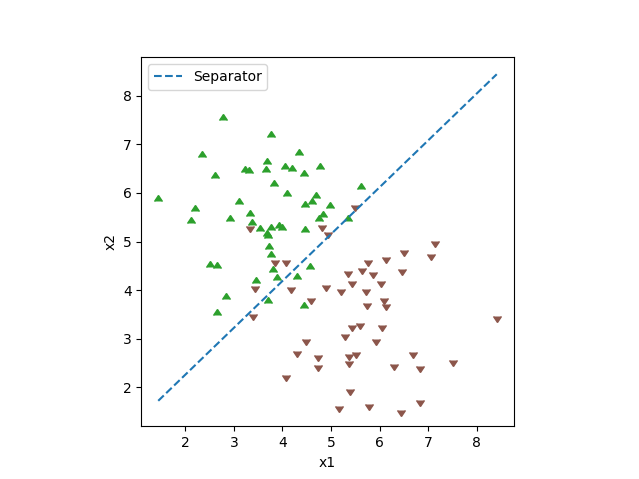
\includegraphics[width=.7\linewidth]{/home/mridul/scai/ml/hw1/src/q3/log_reg.png}
\caption{\label{fig:org09442ad}Decision Boundary for Logistic Regression}
\end{figure}
\clearpage
\section{Q4}
\label{sec:orgfd67199}
\subsection{Q4(a)}
\label{sec:orgc60505f}
\begin{codebox}
Run as
\begin{verbatim}
$ python four_a.py --data-x path/to/q4x.dat --data-y
path/to/q4y.dat [-scale]
\end{verbatim}
Note, the optional argument \verb|-scale| normalizes the
data, since it was mentioned to normalize data for Q4.
Although, running without it gives the correct result as
well. Values listed below are for runs with \verb|-scale|
enabled.
\end{codebox}
The values of the parameters found are:
\begin{equation*}
\mu_0 = \;
\begin{bmatrix}
-0.16168709\\
0.07834578
\end{bmatrix}
\end{equation*}

\begin{equation*}
\mu_1 = \;
\begin{bmatrix}
0.16168709\\
-0.07834578
\end{bmatrix}
\end{equation*}

\begin{equation*}
\Sigma = \;
\begin{bmatrix}
1.96839477e-04& -5.50137819e-06\\
-5.50137819e-06&  6.93961308e-05
\end{bmatrix}
\end{equation*}
\subsection{Q4(b)}
\label{sec:org588e992}
\begin{codebox}
Run as
\begin{verbatim}
$ python four_b.py --data-x path/to/q4x.dat --data-y
path/to/q4y.dat [-scale]
\end{verbatim}
\end{codebox}
The data plotted is shown in figure \ref{fig:orgd01715b}.
\begin{figure}[!ht]
\centering
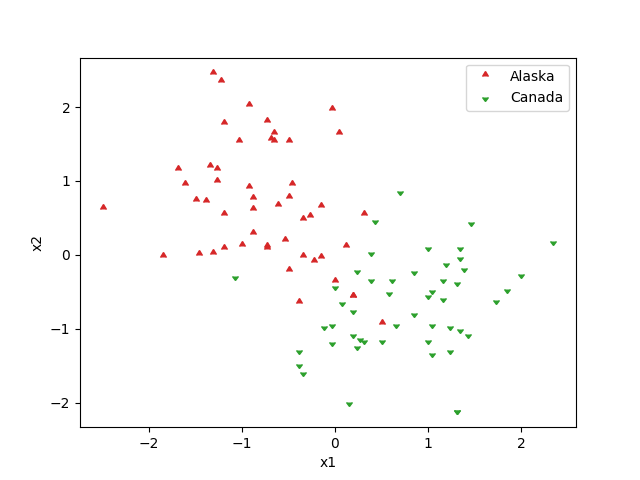
\includegraphics[width=.8\linewidth]{/home/mridul/scai/ml/hw1/src/q4/four_b.png}
\caption{\label{fig:orgd01715b}Data}
\end{figure}
\clearpage
\subsection{Q4(c)}
\label{sec:org063d9de}
\begin{figure}[!ht]
\centering
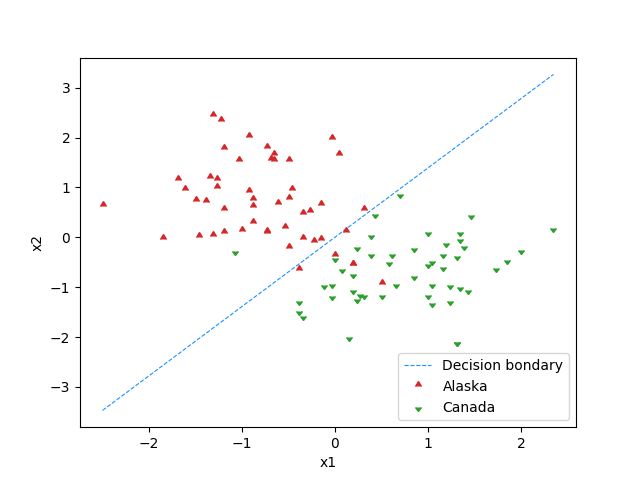
\includegraphics[width=.7\linewidth]{/home/mridul/scai/ml/hw1/src/q4/four_c.png}
\caption{\label{fig:orgf0f2c0a}Linear Decision Boundary by GDA}
\end{figure}
Equation of the linear decision boundary is:
\begin{equation*}
0=(\mu_0-\mu_1)^T\Sigma^{-1}x+\biggl[
\log{\frac{1-\phi}{\phi}}
-\frac{1}{2}\bigl[
\mu_0^T\Sigma^{-1}\mu_0 - \mu_1^T\Sigma^{-1}\mu_1
\bigr]
\biggr]
\end{equation*}
With the values of the parameters in place and with \(x=[x_1\; x_2]^T\):
\begin{equation}
0=-6.39488462\times10^{-13}-1583.23388368x_1+2132.41855595x_2
\end{equation}
\subsection{Q4(d)}
\label{sec:org1f9433b}
\begin{codebox}
Run as
\begin{verbatim}
$ python four_d.py --data-x path/to/q4x.dat --data-y
path/to/q4y.dat [-scale]
\end{verbatim}
\end{codebox}
The values of the parameters obtained are
\begin{equation*}
\mu_0 = \;
\begin{bmatrix}
-0.16168709\\
0.07834578
\end{bmatrix}
\end{equation*}

\begin{equation*}
\mu_1 = \;
\begin{bmatrix}
0.16168709\\
-0.07834578
\end{bmatrix}
\end{equation*}

\begin{equation*}
\Sigma_0 = \;
\begin{bmatrix}
3.49739714e-04& -7.58242443e-05\\
-7.58242443e-05&  1.69417922e-04
\end{bmatrix}
\end{equation*}

\begin{equation*}
\Sigma_1 = \;
\begin{bmatrix}
4.37618193e-04& 5.38187315e-05\\
5.38187315e-05& 1.08166601e-04
\end{bmatrix}
\end{equation*}
\subsection{Q4(e)}
\label{sec:org88a0269}
\begin{codebox}
Run as
\begin{verbatim}
$ python four_e.py --data-x path/to/q4x.dat --data-y
path/to/q4y.dat [-scale]
\end{verbatim}
\end{codebox}
\begin{figure}[!ht]
\centering
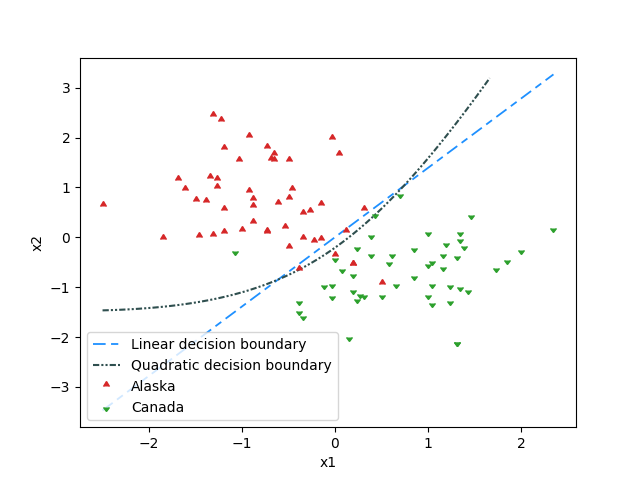
\includegraphics[width=.7\linewidth]{/home/mridul/scai/ml/hw1/src/q4/four_e.png}
\caption{\label{fig:orgb252f3d}Quadratic and Linear Decision Boundary for GDA}
\end{figure}
The equation of the decision boundary with parameter values substituted is:
\begin{equation*}
-3310.73x_2^2 + 732.49x_1^2 + 5256.53x_1x_2 - 2500.63x_2 + 1778.77x_1 - 67.57 =0
\end{equation*}
\par
To get the equation of the decision boundary when
\(x\in\mathbb{R}^2\) I'll begin here:
\begin{equation}
P(y=1|x;\theta)=\frac{1}{1+\frac{P(x|y=0;\theta)P(y=0;\theta)}{P(x|y=1;\theta)P(y=1;\theta)}}
\end{equation}
As in the lecture, we want \(P(y=1|x;\theta)=0.5\). And taking
\(A=\frac{P(x|y=0;\theta)P(y=0;\theta)}{P(x|y=1;\theta)P(y=1;\theta)}\),
this implies \(\log A=0\).
\begin{align*}
A &=
\frac{1-\phi}{\phi}\times\frac{(2\pi)^{-\frac{n}{2}}\lvert\Sigma_0\rvert^{-0.5}\exp(-0.5(x-\mu_0)^T\Sigma^{-1}_0(x-\mu_0))}{(2\pi)^{-\frac{n}{2}}\lvert\Sigma_1\rvert^{-0.5}\exp(-0.5(x-\mu_1)^T\Sigma^{-1}_1(x-\mu_1))}\\
\log A &= \log\Biggl[\frac{1-\phi}{\phi}\frac{\lvert\Sigma_1\rvert^{\frac{1}{2}}}{\lvert\Sigma_0\rvert^{\frac{1}{2}}}\Biggr]-\frac{1}{2}\bigl((x-\mu_0)^T\Sigma^{-1}_0(x-\mu_0)-(x-\mu_1)^T\Sigma^{-1}_1(x-\mu_1)\bigr)
\end{align*}
Taking the first log term there as \(k\).
\begin{equation*}
\log A = k - \frac{1}{2}\bigl(
x^T\Sigma^{-1}_0x-2\mu_0^T\Sigma^{-1}_0x+\mu_0^T\Sigma^{-1}_0\mu_0
-\bigl[
x^T\Sigma^{-1}_1x-2\mu_1^T\Sigma^{-1}_1x+\mu_1^T\Sigma^{-1}_1\mu_1
\bigr]
\bigr)
\end{equation*}
Adding the constants together

\begin{align*}
a &= k - \frac{1}{2}\bigl[
\mu_0^T\Sigma_0^{-1}\mu_0
-
\mu_1^T\Sigma_1^{-1}\mu_1
\bigr]\\
\log A &= a - \frac{1}{2}\bigl[
x^T\Sigma_0^{-1}x - x^T\Sigma_1^{-1}x
-2\bigl(
\mu_0^T\Sigma_0^{-1}x - \mu_1^T\Sigma_1^{-1}x
\bigr)
\bigr]
\end{align*}
This was all general, but now for the two-dimensional, data, we know
that the covariance matrices are \(\mathbb{R}^{2\times 2}\) and the mean vector
is \(\mathbb{R}^{2\times 1}\). Also,
\(\mu_i^T\Sigma_i^{-1}\in\mathbb{R}^{1\times 2}\) for
\(i\in\{0,1\}\). Using more notations:
\begin{equation*}
\Sigma_0^{-1}-\Sigma_1^{-1}=
\begin{bmatrix}
\alpha&\beta\\
\gamma&\delta
\end{bmatrix}
\end{equation*}
\begin{equation*}
\mu_0^T\Sigma_0^{-1}-\mu_1^T\Sigma_1^{-1}=
\begin{bmatrix}
\varphi&\pi
\end{bmatrix}
\end{equation*}
\begin{equation*}
x=
\begin{bmatrix}
x_1\\
x_2
\end{bmatrix}
\end{equation*}

Let \(b=2a\), \(\log A=0\)
\begin{equation*}
0 = b - \alpha x_1^2 - (\gamma + \beta)x_1 x_2 - \delta x_2^2 + 2\varphi x_1 +2\pi x_2
\end{equation*}
At \(x=t\), we can set
\begin{align*}
P =&\; -\delta\\
Q =&\; 2\pi - (\gamma+\beta)t\\
R =&\; 2\varphi t+b-\alpha t^2\\
&\text{such that}\\
0 =&\; Px_2^2+Qx_2+R\\
&\text{and}\\
x_2 =&\; \frac{-Q\pm \sqrt{Q^2-4PR}}{2P}
\end{align*}

This is used in the program to calculate the \(x_2\) coordinate for
given \(x_1\) coordinate to plot the graph. We get two values for
\(x_2\) for a give \(x_1\), corresponding to points where the
probability of sample being in each class is
\(\displaystyle\frac{1}{2}\). I only plot the one that would be
visible in the graph based on the y-axis limits produced by the linear separator.
\subsection{Q4(f)}
\label{sec:org2efb49c}
The quadratic separator believes that as \(x_1\) decreases, \(x_2\)
has to decrease much slower for the fish to still belong to class
\lq\lq Alaska\rq\rq. The linear separator is more biased towards a
simpler decision boundary. The quadratic separator has more power
to fit complicated data. This power is visible in the better fit when
compared with the linear separator. In this situation I see three more
points on the correct side of the curve in exchange of letting go of
one that was being classified correctly before to the wrong side.
\end{document}
